\newpage
\section{Simulation Analysis}
\label{sec:simulation}
\subsection{Simulation for t < 0}
\noindent
The first part of this section covers the simulation of the circuit in ngspice for t < 0.
The values obtained, by ngspice, for currents flowing in each resistance or capacitor(Ampers) and nodes voltages (Volts) are showed in the following table:
\begin{table}[h!]
  \centering
  \begin{tabular}{|c|c|}
    \hline    
    {\bf Name} & {\bf Value [A or V]} \\ \hline
    @cb[i] & 0.000000e+00\\ \hline
@ce[i] & 0.000000e+00\\ \hline
@q1[ib] & 7.022567e-05\\ \hline
@q1[ic] & 1.404513e-02\\ \hline
@q1[ie] & -1.41154e-02\\ \hline
@q1[is] & 5.765392e-12\\ \hline
@rc[i] & 1.411536e-02\\ \hline
@re[i] & 1.411536e-02\\ \hline
@rf[i] & 7.022567e-05\\ \hline
@rs[i] & 0.000000e+00\\ \hline
v(1) & 0.000000e+00\\ \hline
v(2) & 0.000000e+00\\ \hline
base & 2.254108e+00\\ \hline
coll & 5.765392e+00\\ \hline
emit & 1.411536e+00\\ \hline
vcc & 1.000000e+01\\ \hline

  \end{tabular}
  \caption{Operating point. A variable preceded by @ is of type {\em current}
    and expressed in Ampere; other variables are of type {\it voltage} and expressed in
    Volt. (g in "gib" refers to the Ngspice notation of a current source controlled by a voltage).}
  \label{tab:op}
\end{table}

\newpage
\subsection{Simulation for t = 0}
The second section covers the simulation of the circuit for t = 0, where the capacitor is replaced with a voltage source, $v_c$ = V(6) - V(8) (V(6) and V(8) are the values obtained in the previous section). This happens because the voltage of the capacitor ($v_c$) when t < 0 is the same when t = 0. However, V(6) and V(8) are not necessarily the same. Therefore, the capacitor is replaced with the voltage source (initial voltage of the capacitor) so that the boundary conditions V(6) and V(8) can be obtained.
\begin{table}[h!]
  \centering
  \begin{tabular}{|c|c|}
    \hline    
    {\bf Name} & {\bf Value [A or V]} \\ \hline
    zout & 7.866317e+00\\ \hline

  \end{tabular}
  \caption{Operating point. A variable preceded by @ is of type {\em current}
    and expressed in Ampere; other variables are of type {\it voltage} and expressed in
    Volt. (g in "gib" refers to the Ngspice notation of a current source controlled by a voltage).}
  \label{tab:op2}
\end{table}
\newpage
\subsection{Natural response simulation}
The third section covers the simulation of the natural response of the circuit in the interval [0;20] ms, using the boundary conditions obtained in the second section (V(6) and V(8)).
\begin{figure}[h!] \centering
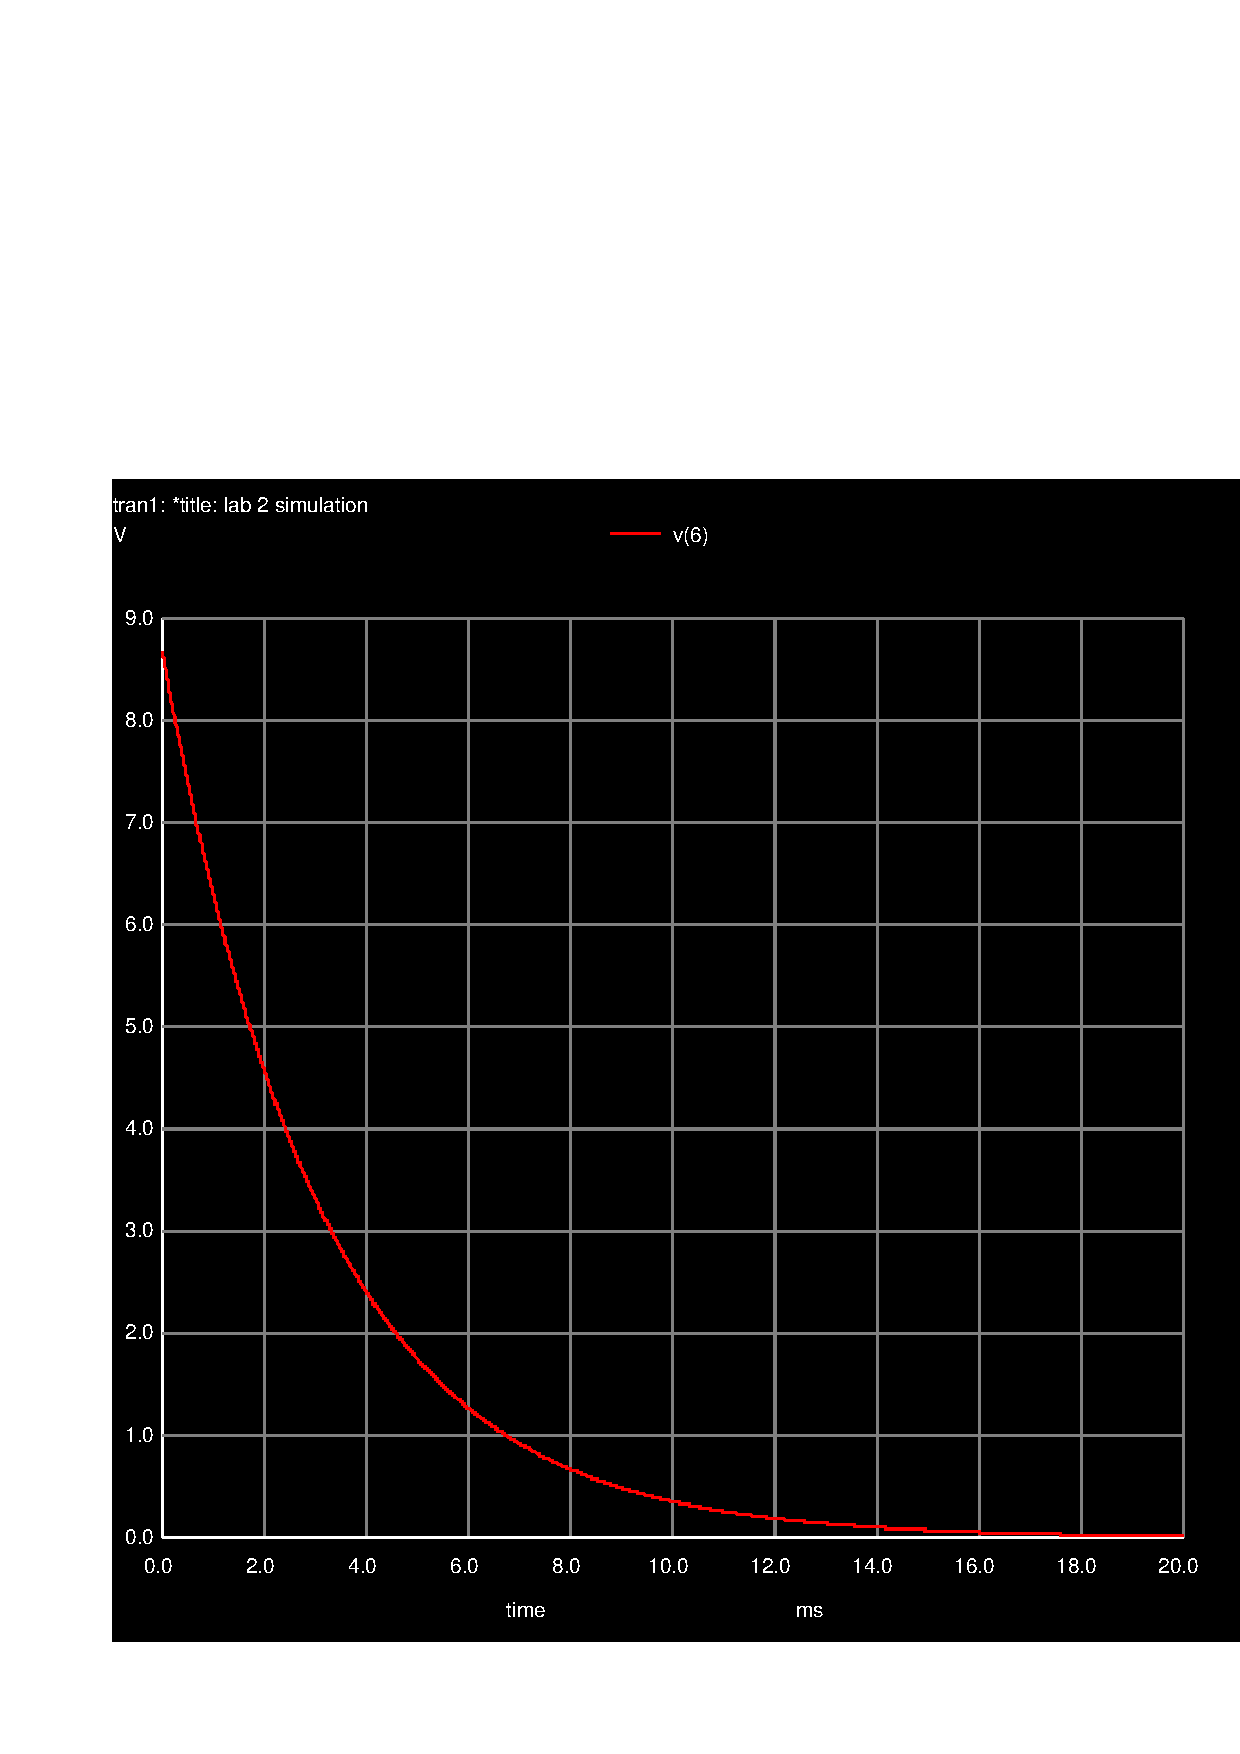
\includegraphics[width=7cm]{../sim/trans.pdf}
\caption{Natural response of $v_6$.}
\label{fig:trans}
\end{figure}
\newpage
\subsection{Total response simulation}
In the forth section, the total response (natural and forced response) is simulated on node 6 in the same interval as the third section, with a given frequency f = 1kHz.
\begin{figure}[h!] \centering
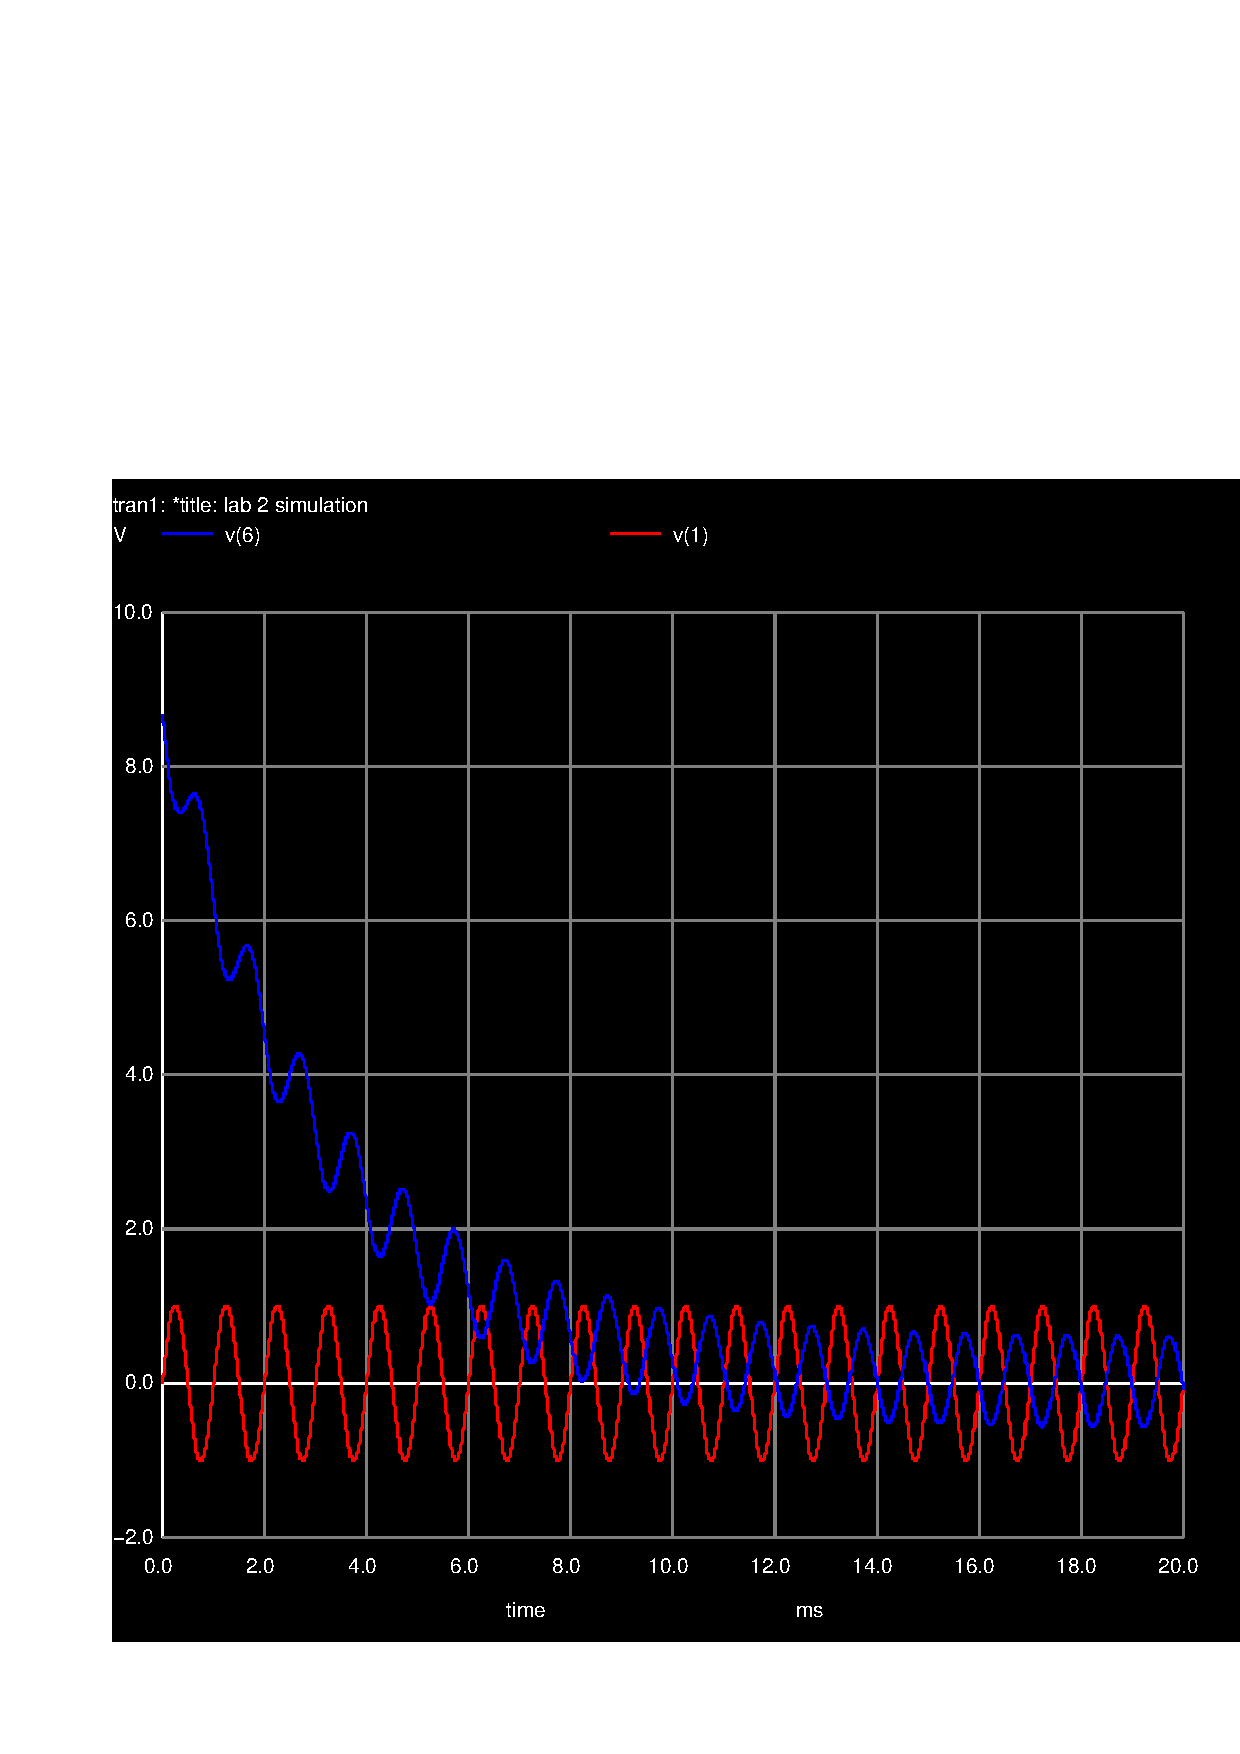
\includegraphics[width=7cm]{../sim/trans2.pdf}
\caption{Total response of $v_6$ and $v_s$.}
\label{fig:trans2}
\end{figure}
\newpage
\subsection{Total response simulation}
In the fifth section, the frequency response is simulated on node 6 (frequency log scale with magnitude in dB, phase in degrees) for the frequency range 0.1 Hz to 1 MHz. The results show that $v_s$(f) stays constant, whereas $v_6$(f) is monotonically decreasing (it decreases 180 degrees in the phase graph and aproximately 6 dB in the magnitude graph). These results derivate from the fact that $v_s$ is the source of the frequency (it will be zero for magnitude graph and 90 for the phase graph) and $v_6$ is an output voltage that is dependent on the frequency source $v_s$.

\begin{figure}[h!] \centering
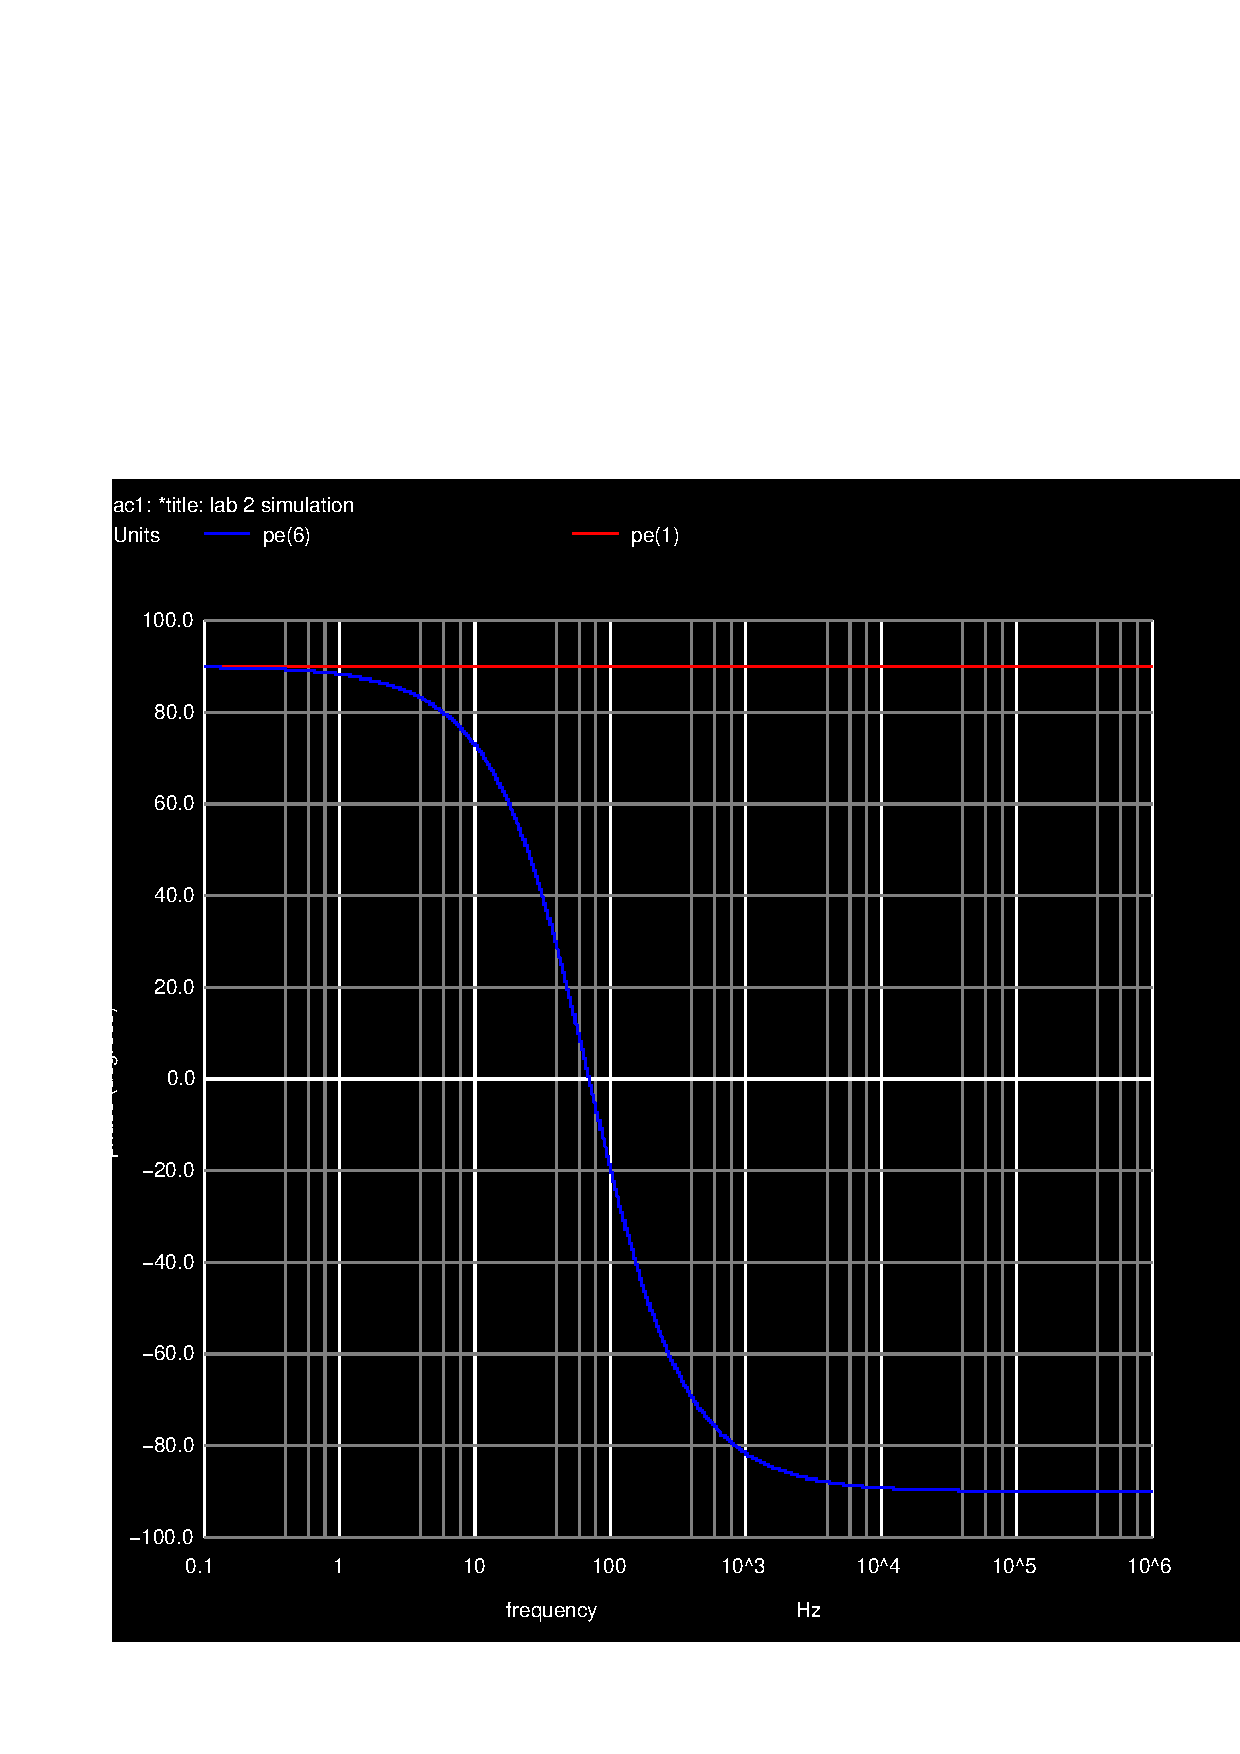
\includegraphics[width=8cm]{../sim/acp.pdf}
\caption{Phase graph for $v_6$ and $v_s$.}
\label{fig:phase}
\end{figure}

\begin{figure}[h!] \centering
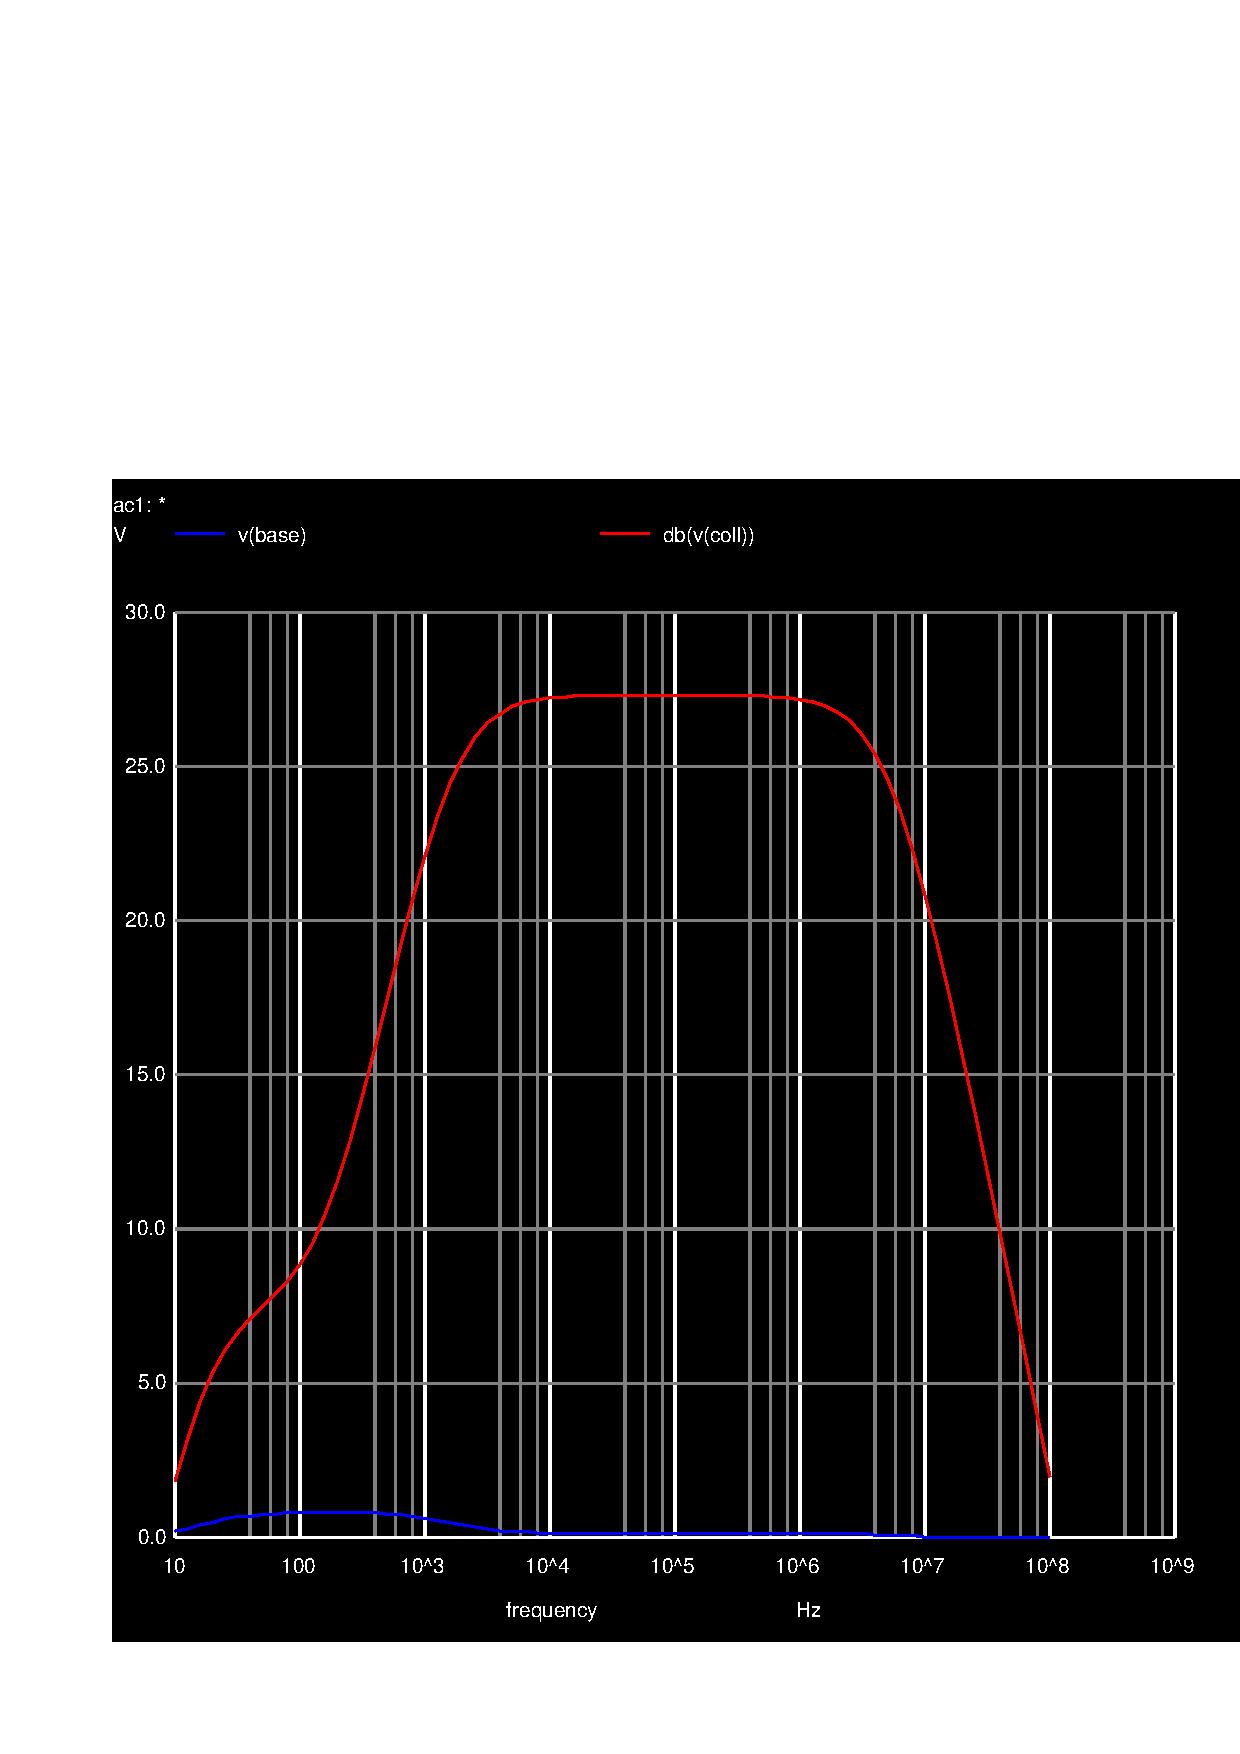
\includegraphics[width=8cm]{../sim/acm.pdf}
\caption{Magnitude graph for $v_6$ and $v_s$.}
\label{fig:magnitude}
\end{figure}





